\section{Optimal Control of Pitch/Travel without Feedback}\label{sec:prob2}

\subsection{State space model}
From the model equations in \eqref{eq:model} we get the continuous state space equation
\begin{equation*}
	\begin{bmatrix}
		\dot{\lambda}\\
		\ddot{\lambda}\\
		\dot{p}\\
		\ddot{p}
	\end{bmatrix} = 
	\begin{bmatrix}
		0 & 1 & 0 & 0 \\
		0 & 0 & -K_2 & 0 \\
		0 & 0 & 0 & 1 \\
		0 & 0 & -K_1K_{pp} & -K_1K_{pd}
	\end{bmatrix}
	\begin{bmatrix}
		\lambda	\\
		\dot{\lambda}		\\
		p		\\
		\dot{p}
	\end{bmatrix} +
	\begin{bmatrix}
		0 \\
		0 \\
		0 \\
		K_1K_{pp} \\
	\end{bmatrix}
	p_c
\end{equation*}

or, alternatively
\begin{equation*}
	\begin{bmatrix}
		\dot{\lambda}\\
		\ddot{\lambda}\\
		\dot{p}\\
		\ddot{p}
	\end{bmatrix} = 
	\begin{bmatrix}
		0 & 1 & 0 & 0 \\
		0 & 0 & -0.0663 & 0 \\
		0 & 0 & 0 & 1 \\
		0 & 0 & -5.3095 & -0.9481
	\end{bmatrix}
	\begin{bmatrix}
		\lambda	\\
		\dot{\lambda}		\\
		p		\\
		\dot{p}
	\end{bmatrix} +
	\begin{bmatrix}
		0 \\
		0 \\
		0 \\
		5.3095 \\
	\end{bmatrix}
	p_c
\end{equation*}

However, in an effort to achieve a more accurate model, alternative state space equations are developed from estimated transfer functions based on measured step response output.

Discuss: 2 pole vs 3 pole, include transfer functions...Not exactly sure exactly what decided on, and how the model got these parameters...

\begin{equation}
	\begin{bmatrix}
		\dot{\lambda}\\
		\ddot{\lambda}\\
		\dot{p}\\
		\ddot{p}
	\end{bmatrix} = 
	\begin{bmatrix}
		0 & 1 & 0 & 0 \\
		0 & -0.03 & -0.39 & 0 \\
		0 & 0 & 0 & 1 \\
		0 & 0 & -7.13 & -3.6
	\end{bmatrix}
	\begin{bmatrix}
		\lambda	\\
		\dot{\lambda}		\\
		p		\\
		\dot{p}
	\end{bmatrix} +
	\begin{bmatrix}
		0 \\
		0 \\
		0 \\
		6.74 \\
	\end{bmatrix}
	p_c
	\label{eq:sys}
\end{equation}

Discuss differences with textbook model

\subsection{Discretization}
Let $x = \begin{bmatrix}\lambda&\dot{\lambda}&p&\dot{p}\end{bmatrix}^\top$, $u = p_c$, and $A_c$, $B_c$ denote the state transition matrix and the **(Whatever B is called)** from \eqref{eq:sys} respectively. Then, discretizing \eqref{eq:sys} using forward Euler with a time step $\Delta t$ we get the discrete time state space model

\begin{subequations}
\label{eq:dmodel}
\begin{align}
	x_{k+1} &= x_k + \Delta t \dot{x_k} \\
			&= x_k + \Delta t (A_c x_k + B_c u_k)\\
			&= (I + \Delta t A_c) x_k + (\Delta t B_c) u_k \\
			&= A x_k + B u_k
\end{align}
\end{subequations}

where $x_k = x(k\Delta t)$ and $u_k = u(k\Delta t)$.

\subsection{Optimal trajectory}

We calculate the trajectory from $x_0 = \begin{bmatrix}\lambda_0&0&0&0\end{bmatrix}^\top$ to $x_f = \begin{bmatrix}\lambda_f&0&0&0\end{bmatrix}^\top$ minimizing the objective function 
\begin{equation}
\label{eq:QC_p}
	\phi = \sum_{i=1}^{N}(\lambda_i - \lambda_f)^2 + qp^2_{c_i}, \quad q \ge 0,
\end{equation}
for a chosen $q$ penalizing input expendature in favour of minimizing deviations in the travel trajectory, and vice verca for $q < 1$. (Copied prev eq from assignment, but are the indexes correct?) Equivalently we can define \eqref{eq:QC_p} in terms of the full state and input variables.

\begin{equation}
	\label{eq:QC_p_QR}
	\phi = \frac{1}{2}\sum_{i=0}^{N-1} (x_{i+1}-x_f)^\top Q (x_{i+1}-x_f) + u_i^\top R u_i,
\end{equation}

where
\begin{equation*}
Q = \begin{bmatrix}2&0&0&0\\0&0&0&0\\0&0&0&0\\0&0&0&0\end{bmatrix}, \ R = 2q.
\end{equation*}

We need to choose different symbols than Q,R, but I don't know which...

The system dynamics \eqref{eq:dmodel} subjects \eqref{eq:QC_p_QR} to the linear equality constraints

\begin{equation}
	\label{eq:eq_constraints}
	\left[\begin{array}{cccc | ccccc}
	I	&&&&			-B	&&&			\\
	-A	&\ddots&&&			&\ddots&&	\\
		&\ddots&\ddots&&	&&\ddots&	\\
		&& -A & I&			&&& -B		\\
	\end{array}\right]
\begin{bmatrix} x_1 \\ \vdots \\ x_N \\ u_0 \\ \vdots \\ u_{N-1} \end{bmatrix}
=
\begin{bmatrix}
-A x_f \\ 0 \\ \vdots \\ 0      
\end{bmatrix}.
\end{equation}

If we let $z = \begin{bmatrix} x_1 & \dots & x_N & u_0 & \dots & u_{N-1} \end{bmatrix}^\top$ and define
\begin{equation*}
	G =
	\begin{bmatrix}
	Q	&&&&&		\\
		&\ddots&&&&	\\
		&&Q&&&		\\
		&&&R&&		\\
		&&&&\ddots&	\\
		&&&&&R		\\
	\end{bmatrix},
\end{equation*}

we can then state the QP-problem in terms of the optimization variable $z$:
\begin{equation*}
	\min_z \ \frac{1}{2} z^\top G z, \quad \textrm{s.t}\ A_{eq} z = B_{eq},
\end{equation*}

with $A_{eq}$, $B_{eq}$ given by \eqref{eq:eq_constraints}. In addition to the equality constraints, we impose lower and upper bounds on the pitch state and controller set-point:

\begin{equation*}
	|p_k| \le \frac{30 \pi}{180}, \quad k \in \{1, \dots, N\},
\end{equation*}

and solve the resulting system using MATLAB's \texttt{quadprog}. The optimal input sequence $u^*$ is applied to the plant in an open loop with results show in figure \ref{fig:opt_openloop}, with the measured trajectory compared to the calculated optimal trajectory $x^*$.

\subsection{Results and discussion}

\begin{figure}[hp]
	\centering
		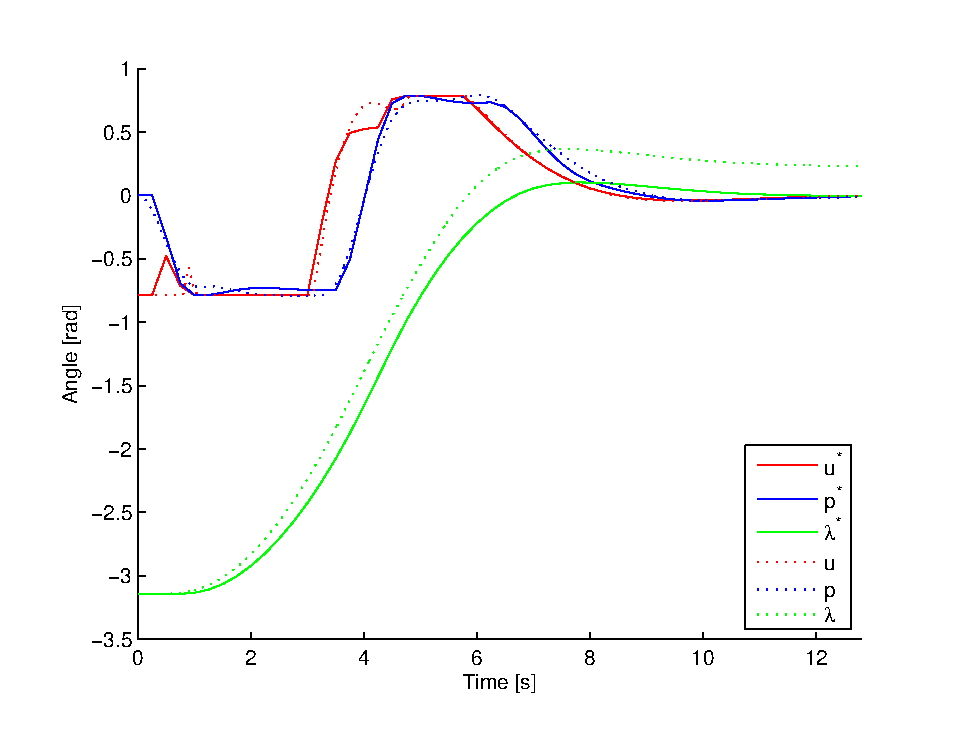
\includegraphics[width=1.00\textwidth]{figures/2/opt_vs_meas_traj.eps}
	\caption{Optimal vs. measured trajectory and input sequence.}
	\label{fig:opt_openloop}
\end{figure}

Opt. input vs measured input discrepency due to interpolation stuff...?

